In this section, we study arithmetic applications of Conjecture \ref{conj_4}, focusing on when we can use this conjecture to force positive rank for families of elliptic curves. In particular we describe a result introduced in \cite{DEW1} that provides a test for forcing rank growth. We call this a Norm Relations test. As we will observe, this test depends only on local arithmetic data associated to the elliptic curve. 

We also compare this new test to a well-studied method of forcing rank growth, namely by using the Parity Conjecture. As such, we first introduce root numbers and the Parity conjecture, before going on to describe the Norm Relations test and presenting some examples of its use. 

%Some of these applications have already been studied in \cite[\S 3]{DEW1}. %For example, the conjecture allows one to predict non-trivial interplay of the primary parts of the Tate-Shafarevich group of families of elliptic curves, non-trivial Selmer groups, and even positive rank. 

%Interestingly, some of these results appear not to be tractable with other common current methods.
%In later sections, we will aim to show that the product of local factors is indeed a norm in quadratic subextension of the field of values, and the following notation, which expands on Notation \ref{not_contr} will be useful.

%\begin{notation} \label{not_total_contr}
%    Let $F$, $\rho$, $m$ and the fields $F_i,F'_j$ be as in Theorem \ref{thm_positive_rank}. Let $K$ be a subfield of $F$ and $\pp$ a prime of $K$. Then we define
%    $$\contr_\rho(\pp)=\frac{\prod'_i C_{\pp\mid p}(F_i)}{\prod'_j C_{\pp\mid p}(F'_j)},$$
%    where the restricted product is taken over all $F_i$ and $F'_j$ containing $K$.
%    We remark that 
%    $$\frac{\prod'_i C_{E/F_i}}{\prod'_j C_{E/F'_j}}=\prod_p\contr_\rho(p)$$
%    where the product runs over all rational primes. Our strategy is to calculate all $\contr_\rho(p)$ locally first, to then multiply them together. We recall once again that if $p$ is a prime of good reduction of the elliptic curve, then $\contr_\rho(p)=1$, so we will only care about the primes of bad reduction.
%\end{notation}

%{\color{red} If $\Theta$ is the relation in $B(G)$ corresponding to our subfields $F_i$ and $F_j'$, then this is just the same as breaking $C(\Theta)$ into $\prod_p C_{\fP \mid p}(\Theta)$... so is this necessary to introduce?}

\subsection{Root Numbers and The Parity Conjecture}\label{sec_parity}

Root numbers (conjecturally) govern the parity of the rank of an elliptic curve. In this subsection, we briefly discuss root numbers and the parity conjecture. %In $\S\ref{sec_pos_rank}$, we will compare using root number computations to another means of forcing positive rank for an elliptic curve, as described in Theorem \ref{thm_positive_rank}. 
We omit the notation, but descriptions of the completed $L$-functions for $L(E / F, s)$ and $L(E / F, \rho, s)$ can be found in \cite[$\S$2.5]{DEW1}.\\


Let $F$ be a number field and $E / F$ an elliptic curve. The parity conjecture states that the rank of $E / F$ is determined by the global root number $w(E / F) \in \{ \pm 1 \}$, that is

\begin{conj}[Parity conjecture]\label{parity}
    $(-1)^{\rk E / F} = w(E / F).$
\end{conj}

In particular if $w(E / F) = -1$, one has that $\rk E / F$ is odd, and so $\rk E / F > 0$. Therefore the computation of root numbers provides a test for forcing positive rank. We note that parity conjecture follows from assuming BSD and the Hasse--Weil conjecture: 

\begin{conj}[Hasse--Weil conjecture]\label{conj_hasseweil}
    $L(E / F, s)$ has a completed $L$-function 
    $\hat{L}(E / F, s)$ that can be analytically continued to $\bC$ and satisfies the following functional equation:
    \[ \hat{L}(E / F, s) = w(E / F) \hat{L}(E / F, 2- s) .\]
\end{conj}

This is known when $F = \bQ$ due to modularity of elliptic curves. Assuming the Hasse--Weil conjecture, one has that if $w(E / F) = 1$, then $\hat{L}(E / F, s)$ is symmetric under $s \leftrightarrow 2 - s$, and so the order of vanishing at $s = 1$ of $\hat{L}(E / F, s)$ is even. Then $\ord_{s = 1} L(E / F, s) = \ord_{s = 1}\hat{L}(E / F, s)$ and assuming BSD one has that $\rk E / F$ is even. 
The parity conjecture for elliptic curves is known to be true over number fields $F$, assuming finiteness of $|\Sha_{E / F}|$, as proven in \cite{TimVlad}.

The global root number is a product of local root numbers. 
\[ w(E / F) = \prod_v w(E / F_v), \]
taking the product over all places (including infinite ones) of $F$. 
The following proposition details how to compute these root numbers. 

\begin{prop}\cite[Theorem 3.1]{DD-BSD}\label{compute-root}
    Let $F$ be a number field, $F_v$ the completion of $F$ with respect to a place $v$. When $v$ is finite, 
    let $\kappa$ be the residue field of $F_v$. Then the local root number $w(E / F_v)$ is given by 
    \begin{enumerate}[(i)]
        \setlength\itemsep{0em}
        \item $w(E / F_v) = -1$ if $v$ is infinite, or if  $E / F_v$ has split multiplicative reduction,
        \item $w(E / F_v) = 1$ if $E / F_v$ has good reduction, or if $E / F_v$ has non-split multiplicative reduction, 
        \item $w(E / F_v) = \legendre{-1}{\kappa}$ if $E / F_v$ has potentially multiplicative reduction and $\kappa$ has characteristic $\geq 3$, where $\legendre{*}{\kappa}$ is the quadratic residue symbol on ${\kappa}^{\times}$,
        \item $w(E / F_v) = (-1)^{\floor{\frac{v(\Delta_E)|\kappa|}{12}}}$, if $E / F_v$ has potentially good reduction and $\kappa$ has characteristic $\geq 5$, where $\Delta_E$ is the minimal discriminant of $E$.  
    \end{enumerate} 
\end{prop}

\begin{example}[Modular curve $X_1(11)$]
    The elliptic curve $E \colon y^2 + y = x^3  - x^2$ over $\bQ$ has good reduction at $p \not= 11$, and split multiplicative reduction at $p = 11$. Hence by Proposition \ref{compute-root}, $w(E / \bQ) = (-1)(-1) = 1$ and so the parity conjecture implies that $\rk E / \bQ$ is even (actually, it is zero). 
\end{example}

There is also a global root number for the twist of $E$ by an Artin representation $\rho$, denoted $w(E / F, \rho) \in \{ \pm 1 \}$. This appears in a functional equation relating the completed twisted $L$ functions $\hat{L}(E / F, \rho, s)$ and $\hat{L}(E / F, \rho^*, 2 - s)$, where $\rho^*$ is the dual representation of $\rho$. Then one has a parity conjecture for twists by self-dual representations:

\begin{conj}[Parity conjecture for twists]
   Let $\rho$ be a self-dual Artin representation that factors through $\Gal(F / \bQ)$. Then $$ w(E / F, \rho) = (-1)^{\langle \rho, E(F)_{\bC} \rangle}.$$
\end{conj}

Again this is the product of local root numbers; $w(E / F, \rho) = \prod_v w(E / F_v, \rho)$, where $w(E / F_v, \rho) \in \{ \pm 1\}$. The twisted root numbers satisfy the following properties:

\begin{prop}\cite[Lemma A.1, Proposition A.2]{reg-const}\label{compute-root-twist}
    Let $E / F$ be an elliptic curve, $L / F$ a finite Galois extension with Galois group $G$. Let $\rho$, $\tau$ be Artin representations over $F$ that factor through $G$ and let $\trivial$ denote the trivial Artin representation over $F$. Then
    \begin{enumerate}[(i)]
        \setlength\itemsep{0em}
        \item $w(E / F, \rho \oplus \tau) = w(E / F, \rho) w(E / F, \tau)$,
        \item $w(E / F, \trivial) = w(E/ F)$, 
        \item If $H \leq G$ then $w(E / L^H) = w(E/ F, \Ind_{H}^G \trivial)$, 
        \item $w(E / F, \rho \oplus \rho^*) = 1$.
    \end{enumerate}
\end{prop}

Therefore, similarly to the $L$-function of $E / F$, one can factor the root number $w(E / F)$ into twisted root numbers.

\subsection{Norm Relations Tests}
We are concerned with the case of predicting positive rank for families of elliptic curves over certain number fields. We illustrate the proof of the main result that predicts positive rank conditional on Conjecture \ref{conj_4}. Let $F$ be a Galois extension over $\QQ$ and let $G=\Gal(F/\QQ)$. Let $E/\QQ$ be an elliptic curve and let $\rho$ be a representation over $G$, which we view as an Artin representation. Then the representation 
$$\bigoplus_{\mathfrak{g}\in\Gal(\QQ(\rho)/\QQ)}\rho^{\mathfrak{g}}$$
has $\QQ$-valued character and therefore\footnote{see Remark \ref{image-of-burnside}} there is some $m\geq 1$ and subfields $F_i, F_j'$ such that 
$$\left(\bigoplus_{\mathfrak{g}\in\Gal(\QQ(\rho)/\QQ)}\rho^{\mathfrak{g}}\right)^m\oplus\bigoplus_j\Ind_{F'_j/\QQ}\mathds{1}=\bigoplus_i\Ind_{F_i/\QQ}\mathds{1}.$$

Assume that $\rk E/F=0$ so that in particular $\langle \rho, E(F)_\CC\rangle_G=0$. Therefore Conjecture \ref{conj_4} implies that 
\begin{equation}\label{eqn_rank}\tag{\textdagger}
    \frac{\prod_i\BSD(E/F_i)}{\prod_j\BSD(E/F'_j)}=\frac{\prod_i\BSD(E,\Ind_{F_i/\QQ}\mathds{1})}{\prod_j\BSD(E, \Ind_{F'_j/\QQ}\mathds{1})}=\left(\prod_{\mathfrak{g}\in\Gal(\QQ(\rho)/\QQ)}\BSD(E,\rho)^{\mathfrak{g}}\right)^m
\end{equation}
and the right-hand side is clearly the $m$-th power of a norm of an element in $\QQ(\rho)$. 

The product of BSD terms on the LHS of \eqref{eqn_rank} involves regulators, the torsion subgroups, the Tate-Shafarevich groups and the terms $C_{E/F}$ which are the product of local factors. Under the assumption that $\rk E/F=0$, the regulators vanish from the product. In general, it is very difficult to deal with the size of the Tate-Shafarevich group for families of elliptic curves, and therefore very difficult to know if the LHS is an $m$-th power the norm of an element in $\QQ(\rho)$. However, not all hope is lost, since Cassels proved the following.

\begin{thm}
    Let $E$ be an elliptic curve over a number field $K$. If $\Sha_{E/K}$ is finite, then $|\Sha_{E/K}|$ is a square.
\end{thm}

Rational squares are not necessarily the norms of general number fields, but they are always norms of quadratic number fields. Furthermore, if $\QQ(\sqrt{D})$ is a quadratic subfield of $\QQ(\rho)$, then the RHS of \eqref{eqn_rank} is also the norm of an element of $\QQ(\sqrt{D})$, and a rational square if $m$ is even. Under the assumption of finiteness of $\Sha$, we know that $|\Sha_{E/F}|$ and $|E(F)_{\tors}|^2$ are rational squares and therefore norms from $\QQ(\sqrt{D})$. The only remaining terms on the LHS of \eqref{eqn_rank} are the product of local factors $C_{E/F_i}$ and $C_{E/F'_j}$. We have therefore proven the following.

\begin{thm}\cite[Theorem 33]{DEW1} \label{thm_positive_rank}
    Suppose Conjecture \ref{conj_4} holds. Let $E/\QQ$ be an elliptic curve, $F/\QQ$ a finite Galois extension with Galois group $G$, $\rho$ an Artin representation over $\bQ$ that factors through $G$ and 
    $$\left(\bigoplus_{\mathfrak{g}\in\Gal(\QQ(\rho)/\QQ)}\rho^{\mathfrak{g}}\right)^m=\bigoplus_i\Ind_{F_i/\QQ}\mathds{1}\ominus\bigoplus_j\Ind_{F'_j/\QQ}\mathds{1}$$
    for some $m\geq 1$ and subfields $F_i,F'_j\subseteq F$. If either $\frac{\prod_i C_{E/F_i}}{\prod_j C_{E/F'_j}}$ is not a norm from some quadratic subfield $\QQ(\sqrt{D})\subseteq\QQ(\rho)$, or if it is not a rational square when $m$ is even, then $E$ has a point of infinite order over $F$.
\end{thm}

This is a remarkable result, since it can predict positive rank for general families of elliptic curves based solely on local data. Let us call applying this theorem a \textbf{norm relations test}.
Following this result, we introduce some notation that will be very useful to compute the local factors $C_{E/F}$.

\begin{notation}\label{not_contr}
    Let $E$ be an elliptic curve defined over $\QQ$ and let $F/K$ be a finite extension of number fields. For each finite place $\pp$ of $K$, we write the \textbf{local contribution of $\pp$} as 
    %$$T_{\mathfrak{P}\mid\pp}(E/F)=\prod_{\mathfrak{P}\mid\pp}c_\mathfrak{P}(E/F)\quad\text{and}\quad D_{\mathfrak{P}\mid\pp}(E/F)=\prod_{\mathfrak{P}\mid\pp}\left|\frac{\Delta_{E,\mathfrak{P}}^{\min}}{\Delta_E}\right|_\mathfrak{P}^{\frac{1}{12}},$$
    $$T_{\mathfrak{P}\mid\pp}(E/F)=\prod_{\mathfrak{P}\mid\pp}c_\mathfrak{P}(E/F),\quad D_{\mathfrak{P}\mid\pp}(E/F)=\prod_{\mathfrak{P}\mid\pp}\left|\frac{\Delta_{E,\mathfrak{P}}^{\min}}{\Delta_E}\right|_\mathfrak{P}^{\frac{1}{12}}$$ 
    and $C_{\fP\mid\fp}(E/F)=T_{\fP\mid\fp}(E/F)D_{\fP\mid\fp}(E/F)$, where the product ranges over primes $\fP$ of $F$ over $\pp$. The local Tamagawa number is defined in $\S$\ref{subs_tamagawa}, $\Delta_E$ is the global minimal discriminant of $E / \bQ$, and $\Delta_{E, \fP}^{\min}$ is the minimal discriminant of $E$ at $\fP$. 

    Thus given $F / K$, one can obtain the global contributions from the terms above by taking the product over all primes $\fp$ of $K$. We denote the \textbf{global contribution over $F$} of the Tamagawa numbers and the discriminant terms as 
    $$T(E/F)=\prod_\pp T_{\fP\mid\pp}(E/F)=\prod_\fP c_\fP(E/F)\quad\text{and}\quad D(E/F)=\prod_\pp D_{\fP\mid\pp}(E/F)=\prod_\fP \left|\frac{\Delta_{E,\mathfrak{P}}^{\min}}{\Delta_E}\right|_\mathfrak{P}^{\frac{1}{12}}.$$ 
An immediate consequence of this notation is the fact that $C_{E/F}=T(E/F)D(E/F)$.
%Observe that if $E$ has good reduction over $\pp$, then $T_{\mathfrak{P}\mid\pp}(E/F)=D_{\mathfrak{P}\mid\pp}(E/F)=1$ for any finite extension $F$ of $K$. 
\end{notation}

We have now seen that both Theorem \ref{thm_positive_rank} and Conjecture \ref{parity} can force the rank of an elliptic curve to be positive. One can observe that for the examples in the next subsection, whenever our norm relations test forces rank growth, a root number computation for the subfields appearing in our relation also implies positive rank. 
It would be a lot more interesting if we could find an example where the norm relations test forces positive rank and root numbers do not. 
We suspect however that such an example does not exist. 

Consider $G = \Gal(L / K)$. Then changes in parity between subfields of $L / K$ correspond to twisted root numbers being equal to $-1$. Indeed by Proposition \ref{compute-root-twist}, for $H \leq G$, 
\[ \Ind_{H}^G \trivial \simeq \trivial\oplus \bigoplus_i \rho_i  \implies w(E / L^H) = w(E / K)\prod_i w(E / K, \rho_i) \] for some representations $\rho_i $ of $G $. Hence a change in parity from $w(E / K)$ to $w(E / L^H)$ is determined by $\prod_i w(E / K, \rho_i)$. On the premise that a failure of our norms relations test is always explained by root numbers, we conjecture the following:
%{\color{red} On the other hand ... root numbers should help us determine what the regulators look like ... and we could put them into our factors... maybe talk about this in a conclusion / outlook?}

\begin{conj}
Consider an elliptic curve $E / \bQ$, $F / \bQ$ a finite Galois extension, and relation 
$$\left(\bigoplus_{\mathfrak{g}\in\Gal(\QQ(\rho)/\QQ)}\rho^{\mathfrak{g}}\right)^m=\bigoplus_i\Ind_{F_i/\QQ}\mathds{1}\ominus\bigoplus_j\Ind_{F'_j/\QQ}\mathds{1}$$
as in Theorem \ref{thm_positive_rank}. If the product $\frac{\prod_i C_{E/F_i}}{\prod_j C_{E/F'_j}}$ is not a norm from some quadratic subfield $\QQ(\sqrt{D})\subseteq\QQ(\rho)$, or if it is not a rational square when $m$ is even, then there exists a self-dual Artin representation $\tau$ of $G$ such that $w(E / \bQ, \tau) = -1 $. 
\end{conj}

The case of odd order Galois groups inspires some confidence in this conjecture. In $\S$\ref{subsec-odd}, we prove that one cannot use Theorem \ref{thm_positive_rank} to conclude that $\rk E / F > 0$, i.e. that our norms relation test never "fails".
The reason one would expect that our norm relations test never forces rank growth in this case is because root number computations do not, as we now show.

\begin{lemma}
 Let $F / \bQ$ be an odd Galois extension with $G = \Gal(F / \bQ)$. Then $w(E / \bQ) = w(E / F^H)$ for all $H \leq G$. 
\end{lemma}

\begin{proof}
Consider $H \leq G$ and intermediate field $F^H$. Then 
$\Ind_H^G \trivial \simeq \trivial \oplus 
\rho \oplus \rho^*$ for some non self-dual representation $\rho$ of $G$, since the only self-dual representation of an odd-order group is the trivial representation. Therefore by Proposition \ref{compute-root-twist}, $w(E / F^H) = w(E / F)w(E, \rho \oplus \rho^*)$ and $w(E, \rho \oplus \rho^*) = 1$. Hence $w(E / \bQ) = w(E / F^H)$ for all $H \leq G$. 
\end{proof}

Therefore once we assume that $\rk E / \bQ = 0$, the parity conjecture tells us that $\rk E / F^H$ is even for all $H \leq G$, which does not force it to be non-zero. 


\subsection{Examples}

We now present some examples where we use Theorem \ref{thm_positive_rank} to force positive rank. Throughout we will consider an elliptic curve $E$ defined over $\bQ$, and a finite Galois extension $F / \bQ$ with Galois group $G = \Gal(F / \bQ)$. We let $\Delta_E$ denote the global minimal differential of $E / \bQ$. 
%As described in Remark \ref{rephrase-thm}, the strategy is to find a representation $\rho$ of $G$ and a $\rho$-relation $\Theta \in \B(G)$ such that $C(\Theta)$ is either not a norm from a quadratic subfield of $\bQ(\rho)$, or not a rational square, as appropriate. 
We start with a small observation:

\begin{rem}[Taking quotients]
   Let $E$, $F$, $G$ be as above. Consider $H \leq G$, and $N \triangleleft G$ such that $N \leq H$. Let $L = F^N$. Then $C_{E / F^H}$ is equal to $C_{E / L^{H/N}}$ as the fields $F^H$ and $L^{H/ N}$ are isomorphic. 
    
%    Consider a representation $\rho$ of $G$ with $N \leq \ker \rho$, so that $\bQ(\rho) = \bQ(\rho^N)$. Then, if $\Theta = \sum_i n_i H_i \in \B(G)$ with $N \leq H_i$ for all $i$, it follows that $N \cdot \Theta / N = \Theta / N$ being a norm relation for $C \colon \B(G / N) \to \bQ^{\times}$ implies that $\Theta$ is a norm relation for $C \colon \B(G) \to \bQ^{\times}$. 
\end{rem}

%We will be computing the terms $C_{E / F^H}$ for $F_i \subset F$ locally. Thus given a prime $p$ and subfield $F_i = F^H$ for 


When computing Tamagawa numbers, we will need to be able to count primes and compute ramification degrees in intermediate extensions of $F / \bQ$, which is described by the following. 

\begin{exercise}[Counting primes and ramification degrees]\label{ex-counting}
Consider a prime $p \in \bQ$ and decomposition and inertia groups $D_p$, $I_p \leq G$. Let $H \leq G$. 
\begin{enumerate}
    \setlength\itemsep{0em}
    \item The number of primes above $p$ in $F^H$ is given by the number of orbits of $D_p$ on $H \backslash G$, where $D_p$ acts by $d(Hg) = H g d^{-1}$ for $d \in D_p$. Equivalently it is $|H \backslash G / D_p|$.
    \item Let a prime $\fP$ above $p$ in $F^H$ correspond to an orbit $Y$ of $D_p$ acting on $H \backslash G$. Then the inertia degree of $\fP$ over $\bQ$ is the size of the $I_p$ sub-orbits on $Y$. 
\end{enumerate}
\end{exercise}


\begin{example}[Brauer relation forces growth]\label{ex-C2C6}
    Let $G = C_2 \times C_6$, with subgroup diagram
    \begin{figure}[H]
        \centering
    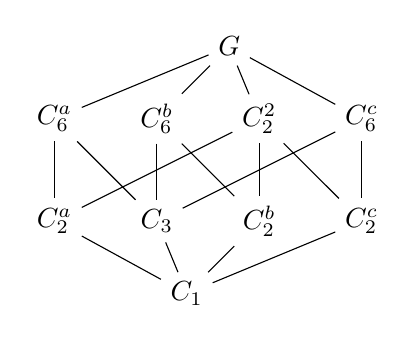
\begin{tikzpicture}[node distance=1.3cm]
        \node(G)[midway]{$G$};
        \node(C6b)[below left of =G]{$C_6^{b}$}; \node(C6a)[left of=C6b]{$C_6^{a}$};  
        \node(C22)[right of=C6b]{$C_2^{2}$};    \node(C6c)[right of=C22]{$C_6^{c}$};
        \node(C2a)[below of=C6a]{$C_2^{a}$};    \node(C3)[below of=C6b]{$C_3$};
        \node(C2b)[below of=C22]{$C_2^{b}$};    \node(C2c)[below of=C6c]{$C_2^{c}$};
        \node(C1)[below left of=C2b]{$C_1$};
        \draw(G)--(C6a);    \draw(G)--(C6b);    \draw(G)--(C6c);    \draw(G)--(C22);
        \draw(C6a)--(C2a);  \draw(C6a)--(C3);
        \draw(C6b)--(C2b);  \draw(C6b)--(C3);
        \draw(C6c)--(C2c);  \draw(C6c)--(C3);
        \draw(C22)--(C2a);  \draw(C22)--(C2b);  \draw(C22)--(C2c);
        \draw(C2a)--(C1);   \draw(C2b)--(C1);   \draw(C2c)--(C1);   \draw(C3)--(C1); 
    \end{tikzpicture}
    \end{figure}
    %There is a Brauer relation coming from the $C_2 \times C_2$-quotient, given by $$\Psi = C_3 - C_6^a - C_6^b - C_6^c + 2G.$$ 
    
    Consider an order $6$ character $\rho_a$ of $G$ with $C_2^{a}$ in its kernel. This has $\bQ(\rho_a) = \bQ(\zeta_6) = \bQ(\sqrt{-3})$. Let $\tau$ generate $\Gal(\bQ(\rho_a) / \bQ)$. One has
    \begin{equation}\label{ex1-rel}\tag{\textdagger}
    \Ind_{C_2^{a}}^G \trivial  \ominus \Ind_{C_6^{a}}^G \trivial \ominus \Ind_{C_2^{2}}^G \trivial \oplus \Ind_G^G \trivial \simeq \rho_a \oplus \rho_a^{\tau} .
    \end{equation}
    Let $E / \bQ$ be a semistable elliptic curve. To apply Theorem \ref{thm_positive_rank}, we need to compute
    \begin{equation}\label{ex1}\tag{*} 
        \frac{C_{E / F^{C_2^a}} C_{E / \bQ} }{C_{E / F^{C_6^a}} C_{E / F^{C_2^2}}} = 
        \frac{C_{E / L} C_{E / \bQ}}{C_{E / L^{C_3}} C_{E / L^{C_2}}}
    \end{equation} 
    where $L = F^{C_2^a}$ has $\Gal(L / \bQ) = C_6$, and check whether it is a norm from $\bQ(\sqrt{-3})$. This is a product of local Tamagawa numbers, as the minimal differential terms are $1$ when $E / \bQ$ is semistable (Lemma \ref{lem_Dterms}(i)). 
    
    One needs to compute these locally for each $p \in \bQ$. If $E / \bQ_p$ has good reduction, then the Tamagawa numbers at all places above $p$ in the subfields of $L$ are $1$. Suppose that $E / \bQ_p$ has split multiplicative reduction at $p$. Let $n = v_p(\Delta_E)$. For $H \leq G$, the Tamagawa number at a prime $\fP$ above $p$ in $L^H$ is given by $c_{\fp}(E / L^H) = e_{\fP \mid p} n$, where $e_{\fP \mid p}$ is the ramification degree. Thus the computation of Tamagawa numbers depends on the choice of decomposition group $D_p \leq C_6$ (to count the number of primes above $p$ in a given subfield) and the choice of inertia group $I_p \leq C_6$ (to compute the ramification indices). 
    
    The following table describes the product of Tamagawa numbers at places above $p$ in our expression, for varying $D_p$ and $I_p$. We let $T_{\fP \mid p}(E / L^H) = \prod_{\fP \mid p}c_{\fP}(E / L^H)$ for $H \leq \Gal(L / \bQ)$ as defined in Notation \ref{not_contr}. Let $C_p = c_p(E / \bQ)T_{\fP \mid p}(E / L) \big/ T_{\fP \mid p}(E / L^{C_3})T_{\fP \mid p}(E / L^{C_2})$. 
    \[
    \begin{array}{c c c c c c c}
        D_p & I_p & c_p(E / \bQ) & T_{\fP \mid p}(E / L^{C_3}) & T_{\fP \mid p}(E / L^{C_2}) & T_{\fP \mid p}(E / L) & C_p\\ 
        \hline
        C_1 & C_1 & n & n^2 & n^3 & n^6 & \square\\
        C_2 & C_1 & n & n & n^3 & n^3 & \square\\
        C_3 & C_1 & n & n^2 & n & n^2 & \square \\
        C_6 & C_1 & n & n & n & n & \square \\
        C_2 & C_2 & n & 2n & n^3 & (2n)^3 & \square \\
        C_6 & C_2 & n & 2n & n & 2n & \square \\
        C_3 & C_3 & n & n^2 & 3n & (3n)^2 & 3\cdot\square \\
        C_6 & C_3 & n & n & 3n & 3n & \square\\
        C_6 & C_6 & n & 2n & 3n & 6n & \square
    \end{array}
    \]

    In all cases we see that $C_p$, the contribution of Tamagawa numbers above $p$, is a norm form $\bQ(\sqrt{-3})$. It is not too hard to check that this is also the case when $E / \bQ_p$ has non-split multiplicative reduction. Therefore the expression in \eqref{ex1} is always a norm from $\bQ(\rho_a)$. This is an example of a more general phenomenon; for cyclic groups we always get a norm. This follows from  Theorem \ref{thm_consistent_cyclic}, which is proven in \S\ref{sec_cyclic}.
    %and $F / \bQ$ an abelian extension with $G = \Gal(F / \bQ)$. We claim that $C(\Theta) \in \fieldnorm{\rho_a}$, for all such $E$. Since each subgroup in $\Theta$ contains $C_2^{a}$, we have that $C(\Theta)$ equals $C(\Theta / C_2^{a})$ where $\Theta / C_2^{a} \in \B(G / C_2^{a}) = \B(C_6)$.  Now $\Theta / C_2^{a}$ is a $\chi_6$-relation, where $\chi_6 = \rho_a^{C_2^a}$ is a faithful order $6$ character of $C_6$, with $\bQ(\chi_6) = \bQ(\rho_a)$. But for cyclic groups we always get norm relations; by Theorem \ref{thm_consistent_cyclic}, $C(\Theta / C_2^{a}) \in \fieldnorm{\rho_a}$.

    But! Observe that{\footnote{this is called a Brauer relation, see Definition \ref{def-brauer}}} 
    \[ \Ind_{C_3}^G \trivial \ominus \Ind_{C_6^a}^G \trivial \ominus \Ind_{C_6^b}^G \trivial \ominus \Ind_{C_6^c}^G \trivial \oplus (\Ind_G^G \trivial)^{\oplus 2} = 0 \]
    as a virtual permutation representation. Append this to the left hand side of \eqref{ex1-rel}. Then Theorem \ref{thm_positive_rank} asks us to compute 
    \begin{equation}\label{ex1-rel2}\tag{**}
    \left(\frac{C_{E / F^{C_2^a}} C_{E / \bQ} }{C_{E / F^{C_6^a}} C_{E / F^{C_2^2}}}\right) \cdot \left( \frac{C_{E / F^{C_3}} C_{E / \bQ}^2}{C_{E / F^{C_6^a}}C_{E / F^{C_6^b}}  C_{E / F^{C_6^c}} } \right). 
    \end{equation}
    
    We can find instances where the second factor is not a norm from $\bQ(\sqrt{-3})$. Indeed suppose $E / \bQ$ has split multiplicative reduction at a prime $p$ with $D_p = G$, $I_p = C_6^b$. Let $v_p(\Delta_E) = n$. Then there is only one prime above $p$ in each subfield. Suppose $E$ has good reduction at all other primes (or multiplicative reduction at primes that are totally split in $F / \bQ$ would also be fine).
     Then our expression \eqref{ex1-rel2} is equal to
     \[ \frac{(6n)(n)}{(2n) (3n)} \cdot \frac{(2n)(n)^2}{(2n)(n)(2n)} \cdot \square = \frac{1}{2} \cdot \square, \] 
     which is not a norm from $\bQ(\sqrt{-3})$. Hence one must have $\rk E / F > 0$. 
\end{example}

\begin{example}[Dihedral]
    Let $q_1, q_2$ be odd primes. Consider $G = D_{2 q_1 q_2}$ the dihedral group of order $2 q_1 q_2$. 
    Let $\rho$, $\tau_1$, $\tau_2$ be two-dimensional irreducible representations of $G$ corresponding to rotating a $(q_1 q_2)$-gon by $2 \pi / q_1 q_2$, $2 \pi / q_1$, $2 \pi/ q_2$ respectively. These are all self-dual. The Galois conjugates of these representations, as well as the trivial $\trivial$ and sign $\epsilon$, yield all the irreducible representations of $G$. Let 
    \[  \sigma_{\rho} = \bigoplus_{ \fg \in \Gal(\bQ(\rho) / \bQ)} \rho^{\fg}, \qquad
        \sigma_1 = \bigoplus_{ \fg \in \Gal(\bQ(\tau_1) / \bQ)} \tau_1^{\fg}, \qquad
        \sigma_2 = \bigoplus_{ \fg \in \Gal(\bQ(\tau_2) / \bQ)} \tau_2^{\fg}. \]  
    Then $ \{ \trivial , \epsilon, \sigma_{\rho}, \sigma_1, \sigma_2 \}$ are a basis for the irreducible representations of $G$ over $\bQ$. 
    One has
\[
        \Ind_{C_2}^G \trivial \simeq \trivial \oplus \sigma_1 \oplus \sigma_2 \oplus \sigma_{\rho}, \quad
        \Ind_{D_{2 q_1}}^G \trivial \simeq \trivial \oplus \sigma_2, \quad
        \Ind_{D_{2 q_2}}^G \trivial \simeq \trivial \oplus \sigma_1,
\]
% There is an irreducible representation $\rho$ of $G$, obtained by inducing a linear order $q_1 q_2$ faithful representation from $C_{q_1 q_2}$. Thus $\rho$ is of degree $2$ and $\bQ(\rho) = \bQ(\zeta_{q_1 q_2})^{C_2}$. Then $\rho$ has $\frac{(q_1 - 1)(q_2 - 1)}{2}$ Galois conjugates, and so $\repnorm{\rho}$ is of dimension $2 \cdot \frac{(q_1 - 1)(q_2 - 1)}{2}$. 
and so 
\begin{equation*}
\Ind_{C_2}^G \trivial \ominus \Ind_{D_{2 q_1}}^G \trivial \ominus \Ind_{D_{2 q_2}}^G \trivial \oplus \Ind_{G}^G \trivial \simeq \bigoplus_{ \fg \in \Gal(\bQ(\rho) / \bQ)} \rho^{\fg}.
\end{equation*}

    Assume $E / \bQ$ is semistable. Suppose that $E / \bQ_p$ has split multiplicative reduction, with $n = v_p(\Delta_E)$. We compute Tamagawa numbers above $p$ as in the previous example, using the same notation. 
    Corollary \ref{cor-odd-decomp} implies that we always get a norm from the contribution above $p$ whenever the decomposition group is a group of odd-order. In fact we only get a non-square contribution when the decomposition group is $D_{2 q_1}$ or $D_{2 q_2}$ (and $I_p$ is non-trivial). 
     
    For example, let $p$ have decomposition group $D_{2 q_1}$ and inertia group $C_{q_1}$.
    This time, counting primes and computing ramification degrees is a little more awkward, we use Exercise \ref{ex-counting}.
        \begin{itemize}[--]
            \setlength\itemsep{0em}
            \item The action of $D_{2 q_1}$ on $C_2 \backslash G$ yields $1$ orbit of size $C_{q_1}$ (the orbit of the identity) and $\frac{q_2 - 1}{2}$ orbits of size $2q_1$ (coming from $C_2$ acting faithfully on $C_{q_2}$). The size of the inertia sub-orbits is $q_1$. Hence $T_{\fP \mid p}(E / F^{C_2}) = (q_1 n)^{1 + \frac{q_2 - 1}{2}}$.
            
            \item The action of $D_{2 q_1}$ on $D_{2 q_1} \backslash G$ yields the same number of orbits as above, but now the action of $C_{q_1} \leq D_{2 q_1}$ is trivial, so that $T_{\fP \mid p}(E / F^{D_{2 q_1}}) = n^{1 + \frac{q_2 - 1}{2}}$.
            
            \item The action of $D_{2 q_1}$ on $D_{2 q_2} \backslash G$ yields one orbit of size $q_1$, with the inertia sub-orbit also of size $q_1$, hence $T_{\fP \mid p}(E / F^{D_{2 q_2}}) = q_1 n$.
        \end{itemize}
    In total,
    \[ \frac{T_{\fP \mid p}(E / F^C_2) \cdot c_{\fp}(E / \bQ)}{T_{\fP \mid p}(E / F^{D_{2 q_1}})\cdot T_{\fP \mid p}(E / F^{D_{2 q_2}})} = \frac{(q_1 n )^{1 + \frac{q_2 - 1}{2}} (n)}{(n)^{1 + \frac{q_2 - 1}{2}} (q_1 n)} = q_1^{\frac{q_2 - 1}{2}} .\] 
    %By symmetry, taking the decomposition group to be $D_{2 q_2}$ and inertia group $C_{q_2}$, one would obtain $ q_2^{\frac{q_1 - 1}{2}}$.

    So let $E / \bQ$ have split multiplicative reduction at $p$ with decomposition group $D_{2 q_1}$ and inertia group $I_p = C_{q_1}$, and good reduction at all other primes. Further suppose that $q_1, q_2 \equiv 3 \pmod 4$ and that $\legendre{q_1}{q_2} = -1$. Then $\bQ(\sqrt{q_1 q_2}) \subset \bQ(\rho)$ but 
$$\frac{C_{E / F^C_2} C_{E / \bQ}}{C_{E / F^{D_{2 q_1}}} C_{E / F^{D_{2 q_2}}}} = q_1 \cdot \square$$
is not a norm from $\bQ(\sqrt{q_1 q_2})$. Indeed, $q_1$ is not the norm of an element of $\bQ(\sqrt{q_1 q_2})$, since $z^2 q_1 = x^2 - q_1q_2 y^2$ for $x,y,z \in \bZ$ implies $q_1 = \square \pmod {q_2}$, a contradiction. Thus $\rk E / F > 0$.

    This rank growth is predicted by root number computations also, however. Assume that $F / \bQ$ is totally real. Then $w(E / F^H) = (-1)^{[F^H \colon \bQ] + | H \backslash G / D_p|}$ by Proposition \ref{compute-root}. Thus
    \begin{itemize}[--]
        \setlength\itemsep{0em}
        \item $w(E / \bQ) = (-1)^2 = 1$,
        \item $w(E / F^{C_2}) = (-1)^{q_1 q_2} (-1)^{1 + \frac{q_2 - 1}{2}} = (-1)^{\frac{q_2 - 1}{2}}$,
        \item $w(E / F^{D_{2 q_1}}) = (-1)^{q_2}(-1)^{1 + \frac{q_2 - 1}{2}} = (-1)^{\frac{q_2 - 1}{2}},$
        \item $w(E / F^{D_{2 q_2}}) = (-1)^{q_1}(-1) = 1$. 
    \end{itemize}
    Therefore we must have $\rk E / F^{C_2}$, $\rk E / F^{D_{2q_1}} > 0$, so $\rk E / F > 0$. 
    Using the properties in Proposition \ref{compute-root-twist}, the computations of the root numbers for the subfields implies that 
    \[ w\left(E / \bQ, \sigma_1\right) = 1, \quad w\left(E / \bQ, \sigma_2\right) = -1, \quad w\left(E / \bQ, \sigma_{\rho}\right) = 1, \]
  and in particular $w(E / \bQ, \tau_1^{\fg}) = -1$ for some $\fg \in \Gal(\bQ(\tau_1) / \bQ)$.
\end{example}

\begin{example}[Additive reduction example]
Let $G = C_{65} \ltimes C_4$, where $C_4$ acts faithfully on $C_{65}$, as well as the subgroups $C_{13}$ and $C_5$. By inducing a faithful character of order $65$ from $C_{65}$, one obtains a faithful irreducible representation $\rho$ of $G$ of dimension $4$ and with $\bQ(\rho) = \bQ(\zeta_{65})^{C_4}$. In particular one has $\bQ(\sqrt{65}) \subset \bQ(\rho)$. Then
\[ \Ind_{C_4}^G \trivial \ominus \Ind_{C_{13} \ltimes C_4}^G \trivial \ominus \Ind_{C_5 \ltimes C_4}^G \trivial \oplus \Ind_{G}^G \trivial \simeq \bigoplus_{\fg \in \Gal(\bQ(\rho) / \bQ)} \rho^{\fg} .\]
Therefore by Theorem \ref{thm_positive_rank}, either 
\begin{equation}\label{ex3}\tag{\textdagger \textdagger}
\frac{C_{E / F^{C_4}} C_{E / \bQ} }{C_{E / F^{C_{13} \ltimes C_4}} C_{E / F^{C_5 \ltimes C_4}}}
\end{equation}
is a norm from $\bQ(\sqrt{65})$, or $\rk E / F > 0$.  

Suppose $p = 5$ and $E / \bQ_p$ has additive, potentially good reduction. Further suppose that $F / \bQ$ is an extension such that $D_{5} = I_{5} = C_5 \ltimes C_4$ (this is wildly ramified). Let $n = v_p(\Delta_E) < 12$. Then
\begin{itemize}[--]
    \setlength\itemsep{0em}
    \item In $F^{C_4}$ there is one prime above $p$ with ramification degree $5$ and $3$ primes above $p$ with ramification degree $20$,
    \item In $F^{C_{13} \ltimes C_4}$ there is one prime above $p$ with ramification degree degree $5$,
    \item In $F^{C_5 \ltimes C_4}$ there is one prime above $p$ with ramification degree $1$ and $3$ primes above $p$ with ramification degree $4$.
\end{itemize}
Therefore, by Lemma \ref{lem_Dterms}(iii), the product of the minimal differential term is 
\[ \frac{D_{\fP \mid p}(E / F^{C_4}) D_{\fP \mid p}(E / \bQ) }{D_{\fP \mid p}(E / F^{C_{13} \ltimes C_4}) D_{\fP \mid p}(E / F^{C_{5} \ltimes C_4})} = 
\frac{ 5^{\floor{5 n /12}} \cdot \left(5^{\floor{20 n /12}}\right)^3 }{5^{\floor{5 n /12}} \left(5^{\floor{4 n /12}}\right)^3} .\]
If $n = 2$, then this is equal to $5 \mod {(\bQ^{\times})^2}$. By Lemma \ref{tamagawa-num} the Tamagawa number product is
\[ \frac{T_{\fP \mid p}(E / F^{C_4}) T_{\fP \mid p}(E / \bQ) }{T_{\fP \mid p}(E / F^{C_{13} \ltimes C_4}) T_{\fP \mid p}(E / F^{C_{5} \ltimes C_4})} = \frac{1^2 \cdot 3^3 }{1^2 \cdot 3^3} = 1 \text{ or } \frac{1^5}{1^5} = 1.\]

We claim that $5$ is not a norm from $\bQ(\sqrt{65})$. Indeed, $5z^2 = x^2 - 65 y^2$ for $x, y, z \in \bZ$ implies that $5 = \square \pmod 13$, a contradiction since $\legendre{5}{13} = \legendre{13}{5} = \legendre{3}{5} = -1$. Therefore the local contribution of \eqref{ex3} above $5$ is not a norm from $\bQ(\sqrt{65})$. 

What are the local root numbers above $p$? By Proposition \ref{compute-root}, one has
\begin{itemize}[--]
    \setlength\itemsep{0em}
    \item $w(E / \bQ_5) = (-1)^{\floor{ 10 / 12}} = 1$, 
    \item $\prod_{\fp \mid p} w(E /F^{C_4}_{\fp}) = (-1)^{\floor{50 / 12}} \left((-1)^{\floor{200 / 12}}\right)^3 = 1$,
    \item $\prod_{\fp \mid p} w(E /F^{C_{13} \times C_4}_{\fp}) = (-1)^{\floor{50 / 12}} = 1$,
    \item $\prod_{\fp \mid p}w(E /F^{C_{5} \times C_4}_{\fp}) = (-1)^{\floor{ 10/12}}\left((-1)^{\floor{40 / 12}}\right)^3 = -1$ .
\end{itemize}
Hence we see a change in the contributions of local root numbers above $p$ in the intermediate subfields. 




\end{example}
